% 高阶同伦群
\pentry{基本群\upref{HomT3}}

%未完成
%应该是需要大量的图示来直观展示;有动画最好.

%2阶同伦群的想象规则是Jier设计的,期望署名——不署名其实关系也不大,这个规则很简单,估计被独立设计过多次,想署名主要是因为目前为止我没有在任何课本里看到过此规则.

基本群的符号被定义为$\pi_1$.你可能好奇为什么要有一个下标$1$——这是因为基本群只是同伦群中的一种,而仅仅用$\pi_1$群来描述一个拓扑空间往往是不够的.

考虑三个拓扑空间:二维球面(如地球表面)$S^2$,挖去中心的三维球体(如挖去地心的地球)$D^3-x_0$以及$n$维几何空间$\mathbb{R}^n$.容易看出,这三个空间中的任意道路都彼此同伦,因此对任何基点来说都只存在一个回路类,意味着它们的基本群都是平凡群(只有一个元素).这样一来,对于空间中有几个洞、空间的维度是什么等信息就丢失了,我们就需要推广基本群的概念来描述这些性质.这就是高阶同伦群.

\subsection{球和球面}
在$n$维欧几里得空间中,集合$\{(x_1, x_2,\cdots,x_n)|\sum^n_{i=1}x_i^2\leq 1\}$也被称为半径为$1$的$n$维球体,记为$B^n$;集合$\{x_1, x_2, \cdots, x_n|\sum^n_{i=1}x_i^2=1\}$是$B^n$的表面,记为$\partial B^n$,或$S^{n-1}$.记号$\partial B^n$表达的是“$B^n$的边界\upref{Topo0}”,而$S^{n-1}$表达的是“$n$维球面”.

更一般地,所有和球同胚的拓扑空间都被看成球,所有和球面同胚的都被看成球面.比如说,$n$维空间里的“立方体”,$\{(x_1, \cdots, x_n|x_i\in[0, 1],\forall i=1, \cdots, n)\}$,都可以被看成是球.

\begin{theorem}{球面粘接}
对于任意的正整数$n$,把$B^n$表示为一个立方体$\{(x_1, \cdots, x_n|x_i\in[0, 1],\forall i=1, \cdots, n)\}$.$B^n$显然是$\mathbb{R}^n$的子空间.在$B^n$上取一个等价关系$\sim$,使得$B^n$边界上的点都等价,其它点则只和自己等价.则商空间$B^n/\sim$同胚于$S^n$.
\end{theorem}

举个例子,一张平面桌布就是一个$B^2$空间,桌布的边缘是$S^1$;如果把桌布边缘粘合成一个点,那么所得的商空间就是$S^2$.

\subsection{$n$阶回路及其回路积}

基本群是用保基点回路类定义的.由于道路都是区间$I$到拓扑空间的嵌入映射,而回路是首尾相连的,因此一条回路可以看成是$S^1$到拓扑空间的嵌入映射.这时,我们也可以把基本群称作$1$\textbf{阶同伦群}.

类似地,如果把$S^n$嵌入到拓扑空间中,并将道路的首尾相连运算推广到$n$维情况,那么我们还可以得到$n$\textbf{阶同伦群}的定义.

\subsubsection{1阶道路的首尾相连运算}

由\autoref{Topo4_def1}~\upref{Topo4}可知,拓扑空间$X$中的一条道路$p$是从区间$I$到$X$内的一个连续映射.两条道路可以进行首尾相连运算,由\autoref{HomT3_def1}~\upref{HomT3}定义.在这里用图像表示首尾相连运算:


\begin{figure}[ht]
\centering
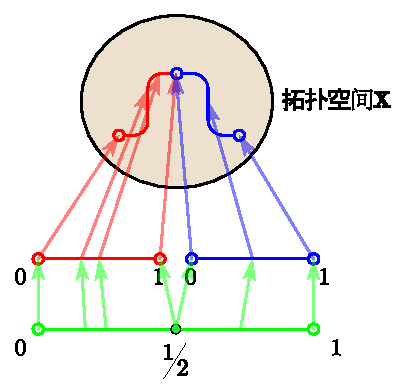
\includegraphics[width=5cm]{./figures/HomT4_1.pdf}
\caption{道路积的示意图.图中红色和蓝色分别表示两条道路,红色道路的终点是蓝色道路的起点.绿色线段也是一个区间$I$,它映射到红蓝区间上后再嵌入到$X$上,其中中点同时映射到红色区间的终点和蓝色区间的终点,这意味着把这两个点粘在一起.} \label{HomT4_fig1}
\end{figure}

如图所示,红色区间到$X$的映射是一条道路,蓝色区间到$X$的映射也是一条道路,它们的首位相连运算所得的道路则是绿色区间映射到红蓝区间后再到$X$的映射.绿色区间也可以看成红蓝区间粘在一起后,进行适当放缩的结果.因此,我们也可以把道路的首尾相连运算看成两个区间粘成一个区间后,再作映射.

\subsubsection{1阶回路的回路积}

继续参考\autoref{HomT4_fig1} ,如果红色道路的起点和终点相同,那么它就是一条回路.回路也可以看成是区间两端粘在一起再嵌入到$X$中,这样起点和终点肯定相同了.因此,回路可以看成是$S^1$到$X$的嵌入映射,它的起点和终点统称\textbf{基点}.

红蓝回路保基点粘接的过程,就是把红色区间的终点和蓝色区间的起点分别解开后再粘到一起,得到绿色区间,然后再把绿色区间的两端粘起来,得到一个绿色的$S^1$,再嵌入$X$.

\begin{figure}[ht]
\centering
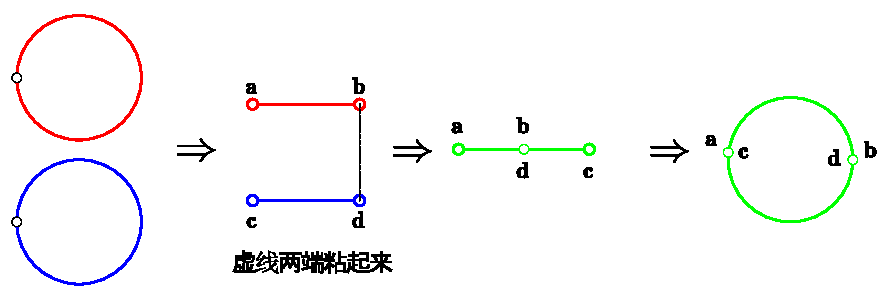
\includegraphics[width=10cm]{./figures/HomT4_2.pdf}
\caption{一维球$S^1$的保基点粘接过程.红蓝$S^1$可以看成是红蓝区间把起点$a, d$和终点$b, c$粘在一起的结果.如果红蓝$S^1$的基点相同(图中分开画了,但是此处认为基点相同),那么可以定义保基点粘接,方法是把基点拆开成起点和终点,然后把红色区间的终点$b$和蓝色区间的起点$d$粘起来,再把红色区间的起点$a$和蓝色区间的终点$c$都粘回基点上.} \label{HomT4_fig2}
\end{figure}

这样粘接的好处是方便想象.在进行保基点同伦变换的时候,你可以想象成基点不动,而道路其它点连续运动,期间保持完整道路的形状以及一直在空间$X$中.把红蓝回路粘接后相当于允许$b$和$d$离开基点运动.

当然,由于道路连通空间中基点的选择不影响基本群的结构,因此我们也可以抽象地把回路的首尾相连看成各自的起始点拆开后再把彼此的首尾相连的过程,图示依然参考\autoref{HomT4_fig2} .

\subsubsection{$2$阶回路的回路积}

$2$阶回路定义为$S^2$到拓扑空间$X$的嵌入映射.类似地,为了方便想象,我们把$S^2$看成正方形$I^2$把四条边都粘成一个点的结果.两条$2$阶回路的粘接过程如图所示:

\begin{figure}[ht]
\centering
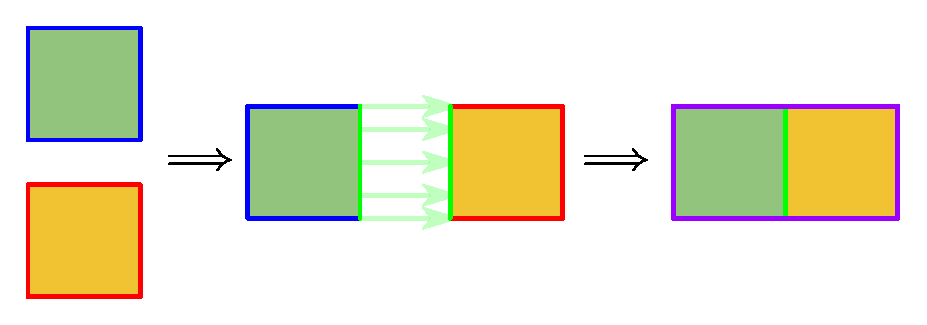
\includegraphics[width=10cm]{./figures/HomT4_3.pdf}
\caption{绿色和黄色正方形分别是两个$D^2$,它们的边界$\partial D^2$分别是蓝色和红色的$S^1$.把蓝色和红色的$S^1$都粘到基点上,那么就得到绿黄两个球面$S^2$.绿黄球面的粘接,就是把绿黄正方形的某一边(亮绿色表示)从基点处解开,然后把亮绿色边粘在一起,但不是粘成一点,而是两条边粘成一边.} \label{HomT4_fig3}
\end{figure}

同样地,这样粘接之后,$2$阶回路的保基点同伦变换就可以想象成红蓝边都限制在基点上,但是亮绿色那一边自由了.我们会在接下来专门用一个小节来讨论想象的方法.%该方法是Jier设计的

\subsubsection{$n$阶回路的回路积}

将$1$、$2$阶回路的粘接方法推广开,就得到$n$阶回路的定义和它们的“首尾相连”运算:

\begin{definition}{$n$阶回路}
给定拓扑空间$X$,则$X$中一个$n$\textbf{阶回路}是$S^n$到$X$的嵌入映射.
\end{definition}

特别地,$1$阶回路又称为回路.

\begin{definition}{$n$阶回路的粘接}
将$S^n$看成超立方体$D^n$将表面$\partial D^n$粘接到一个点的商空间,则两个$S^n$的粘接就是把两个超立方体的某一个超平面解除粘连,然后将这两个平面点对点粘成一个平面.
\end{definition}

为了方便想象,回路的粘接还有一个更抽象的等价定义:

\begin{exercise}{}
两个$S^n$的粘接,就是各取一个道路连通子集$D^n$,将这两个子集的边界$\partial D^n=S^{n-1}$粘成一个$S^{n-1}$,粘连规则是任取一个同胚映射$f:S^{n-1}\rightarrow S^{n-1}$,将$x\in S^{n-1}$和$f(x)$粘在一起.这样粘连以后,再把子集$D^n$挖去,剩下的$S^n$就是球面粘接的结果了.思考这是为什么,图解在下方.
\end{exercise}

以$S^2$的粘接为例,如图所示.

\begin{figure}[ht]
\centering
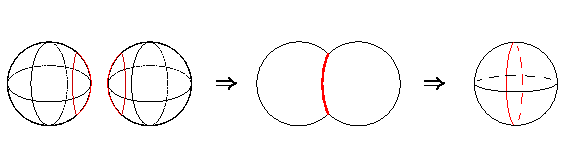
\includegraphics[width=10cm]{./figures/HomT4_4.pdf}
\caption{$S^2$的粘接过程.分别在两个球面上取一小块弧面,弧面的边界用红色表示;将弧面除边界外的部分挖去不用,然后把弧面粘起来,得到一个葫芦表面一样的东西,经过适当的同伦变形得到一个球面.} \label{HomT4_fig4}
\end{figure}

\subsection{高阶同伦群}

\begin{definition}{$n$阶回路类}
设$p_1, p_2:S^n\rightarrow X$是拓扑空间$X$中的两条$n$阶回路,它们都经过基点$x_0\in X$,那么如果$H:S^1\times I\rightarrow X$是$p_1, phi_2$的同伦,并且对于任何$t\in I$,同伦$H$都经过基点$x_0$,那么称$p_1, p_2$是彼此的保基点同伦.按照保基点同伦关系划分的等价类,称为\textbf{回路类}.
\end{definition}

\begin{definition}{$n$阶同伦群}
给定拓扑空间$X$,记其中$n$阶回路的“首尾相连”运算为$*$,则对于回路类$[p_1]$和$[p_2]$,定义其积为$[p_1][p_2]=[p_1*p_2]$.$n$阶回路类的集合配上回路类的积构成一个群,称为$X$上的$n$\textbf{阶同伦群},记为$\pi_n(X)$.
\end{definition}

从$S^n$的粘接过程中我们可以看到,当$n>1$的时候,粘接的方式不唯一,随便取一种同胚都可以进行粘接.这导致了如下深刻的结果\footnote{文献来源:V.A. Vassiliev,《拓扑学导论(中译本)》2.2节,高等教育出版社.}:

\begin{theorem}{同伦群交换性定理}
当$n>1$时,$\pi_n(X)$是阿贝尔群.
\end{theorem}

\subsection{$2$阶同伦群的想象方法}

本小节介绍$2$阶同伦群的想象方法,展示其和基本群的不同和相似之处,希望能帮助读者体会更高阶同伦群的性质.遗憾的是,直观的图示只能应用于$\pi_1$和$\pi_2$群,而$\pi_3$群就已经需要四维空间才能描述,更高阶的同伦群也需要更多的维度.

%未完待续

